\documentclass[a4paper]{article}

%use the english line for english reports
%usepackage[english]{babel}
\usepackage[portuguese]{babel}
\usepackage[utf8]{inputenc}
\usepackage{indentfirst}
\usepackage{graphicx}
\usepackage{verbatim}
\usepackage{listings}
\usepackage{float}


\begin{document}

\setlength{\textwidth}{16cm}
\setlength{\textheight}{22cm}

\title{\Huge\textbf{Xadrersi}\linebreak\linebreak\linebreak
\Large\textbf{Relatório Final}\linebreak\linebreak
\linebreak\linebreak

\includegraphics[scale=0.1]{feup-logo.png}\linebreak\linebreak
\linebreak\linebreak
\Large{Mestrado Integrado em Engenharia Informática e Computação} \linebreak\linebreak
\Large{Programação em Lógica}\linebreak
}

\author{\textbf{Grupo Xadrersi\_1:}\\ António Cunha Seco Fernandes de Almeida - up201505836 \\ João Paulo Madureira Damas - up201504088 \\\linebreak\linebreak \\
 \\ Faculdade de Engenharia da Universidade do Porto \\ Rua Roberto Frias, s\/n, 4200-465 Porto, Portugal \linebreak\linebreak\linebreak
\linebreak\linebreak\vspace{1cm}}
\date{12 de novembro de 2017}
\maketitle
\thispagestyle{empty}

%************************************************************************************************
%************************************************************************************************

\newpage

\section*{Resumo}
Resumo sucinto do trabalho com 150 a 250 palavras (problema abordado, objetivo, como foi o problema resolvido/abordado, principais resultados e conclusões).

\newpage

\tableofcontents

%************************************************************************************************
%************************************************************************************************

%*************************************************************************************************
%************************************************************************************************

\newpage

%%%%%%%%%%%%%%%%%%%%%%%%%%
\section{Introdução}

Descrever os objetivos e motivação do trabalho. Descrever num parágrafo breve a estrutura do relatório.


%%%%%%%%%%%%%%%%%%%%%%%%%%
\section{O Jogo Xadrersi}

\textbf{Origens}\linebreak

Xadrersi é um jogo de tabuleiro para duas pessoas criado por Andi Lewicki, em 2003. Como o nome sugere, surge de uma combinação entre os conhecidos jogos de tabuleiro Xadrez e Reversi.\newline

\textbf{Regras}\newline

O jogo é disputado num tradicional tabuleiro 8x8, inicialmente vazio. A seu dispor, cada jogador possui as peças de que disporia se estivesse numa partida de Xadrez, exceto peões.
Por outras palavras, cada jogador possui um rei, uma rainha, dois cavalos, dois bispos e duas torres.\newline

Os jogadores vão colocando as suas peças no tabuleiro, uma a uma, alternadamente, até todas as peças estarem em jogo.
Após colocada, uma peça não pode ser movida nem retirada (capturada).
No entanto, ataca outras posições do tabuleiro segundo as regras de Xadrez (o rei ataca as posições adjacentes, o bispo diagonalmente, o cavalo em 'L', etc).
Não se aplicam regras de cheque nem afastamento obrigatório entre reis, logo um rei pode ser colocado numa posição onde ficaria em cheque e os reis podem ficar em posições adjacentes. \textit{(Manter ou remover consoante regra estiver implementada?) Os bispos devem ficar em posições de cores opostas, como no Xadrez.}\newline

De uma maneira geral, cada jogada é válida se e só se a peça colocada estiver a ser atacada por pelo menos uma peça adversária. A primeira exceção a esta regra é a primeira jogada, em que não há peças no tabuleiro. O jogador com as peças brancas começa e a primeira peça jogada é obrigatoriamente o rei, podendo ser colocado em qualquer posição.
As figuras \ref{fig:fig1}, \ref{fig:fig2} e \ref{fig:fig3} ilustram uma sequência de jogadas válidas (com as hipóteses em cada turno destacadas) a partir da posição inicial.


\begin{small}
\begin{figure}[H]
\minipage{0.2\textwidth}
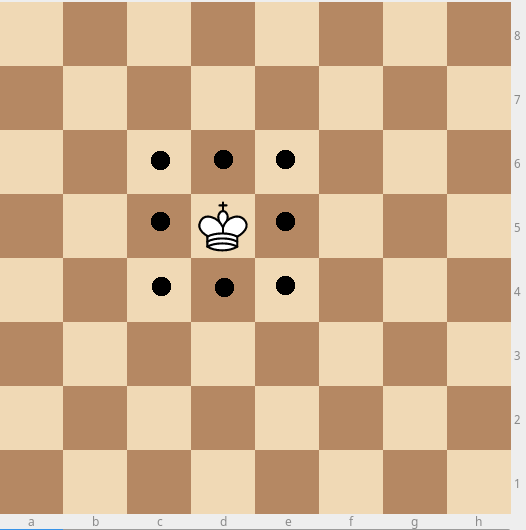
\includegraphics[scale=0.2]{board1.png}
\caption{\textit{Após a primeira jogada, uma peça preta tem de ser colocada adjacentemente ao rei branco de modo a poder ser atacada por este, constituindo uma jogada válida}}
\label{fig:fig1}
\endminipage\hfill
\minipage{0.2\textwidth}
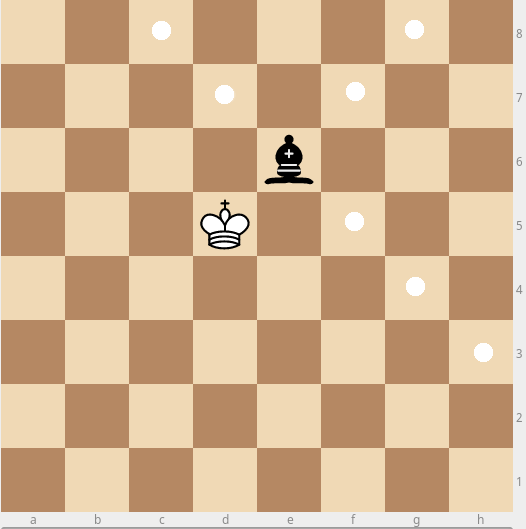
\includegraphics[scale=0.2]{board2.png}
\caption{\textit{Agora, tendo o jogador de peças pretas jogado um bispo, o jogador de peças brancas deve colocar uma peça que intersete o mesmo segundo uma das suas diagonais livres}}
\label{fig:fig2}
\endminipage\hfill
\minipage{0.2\textwidth}
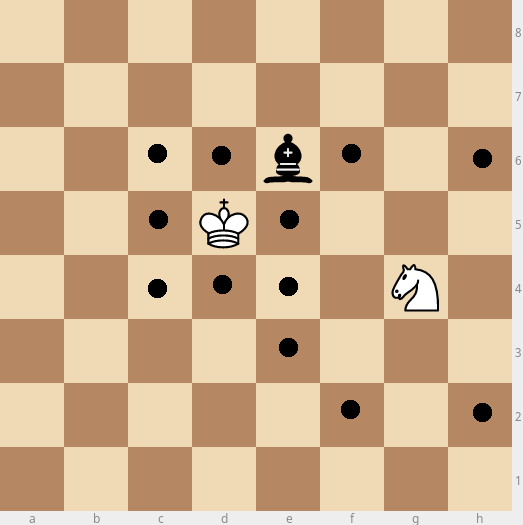
\includegraphics[scale=0.2]{board3.png}
\caption{\textit{Neste caso, tendo já mais do que uma peça branca em jogo, o jogador de peças pretas apenas precisa de se certificar que a peça que colocar é atacada por pelo menos uma peça branca}}
\label{fig:fig3}
\endminipage
\end{figure}
\end{small}


Existe ainda outro caso excecional. Caso seja impossível colocar uma peça de tal modo que seja atacada por uma peça adversária, o jogador pode colocar a peça em qualquer posição livre no tabuleiro. Na figura \ref{fig:fig4} demonstra-se esta situação através de um caso simples.


\begin{figure}[H]
\begin{center}
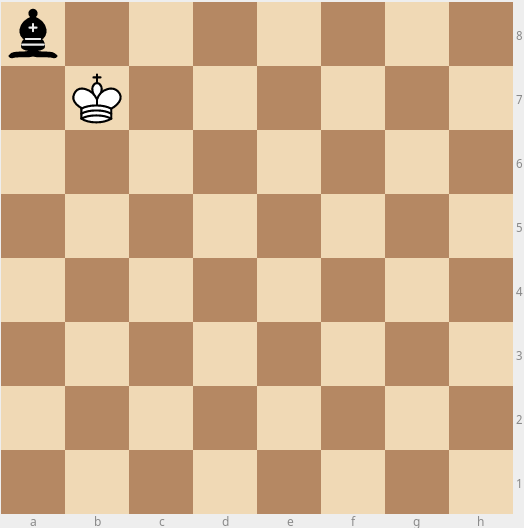
\includegraphics[scale=0.25]{board4.png}
\caption{\textit{Após a jogada inicial do rei, o bispo foi colocado em A8, adjacente ao rei e por isso válido. No entanto, a sua única diagonal está bloqueada e por isso nenhuma posição livre é atacada pelo mesmo. Nesta situação, aplica-se a exceção e a próxima peça branca pode ser colocada em qualquer posição livre.}}
\label{fig:fig4}
\end{center}
\end{figure}


Para além da obrigatoriedade do rei branco ser a primeira peça jogada, existem ainda duas regras adicionais a assinalar para tentar garantir o equilíbrio do jogo:
\begin{itemize}
    \item O rei preto é sempre a última peça a ser colocada no tabuleiro
    \item Quando um jogador coloca em jogo a sua rainha, o outro é obrigado, no turno seguinte, a colocar também a sua rainha em jogo
\end{itemize}

\textbf{Objetivo}\newline

O objetivo é conseguir o maior número de pontos quando o jogo terminar, ou seja, quando todas as peças forem colocadas no tabuleiro.
O número de pontos de um jogador corresponde ao número total de casas que as suas peças atacam.
Caso várias peças ataquem a mesma casa, esta é contabilizada uma vez por cada peça que a ataca.
Existe, por isso, a possibilidade de empate.

%%%%%%%%%%%%%%%%%%%%%%%%%%
\section{Lógica do Jogo}

Descrever o projeto e implementação da lógica do jogo em Prolog, incluindo a forma de representação do estado do tabuleiro e sua visualização, execução de movimentos, verificação do cumprimento das regras do jogo, determinação do final do jogo e cálculo das jogadas a realizar pelo computador utilizando diversos níveis de jogo. Sugere-se a estruturação desta secção da seguinte forma:

\subsection{Representação do Estado do Jogo} Pode ser idêntico ao descrito no relatório intercalar.)

\subsection{Visualização do Tabuleiro} (Pode ser idêntico ao descrito no relatório intercalar.)

\subsection{Lista de Jogadas Válidas} Obtenção de uma lista de jogadas possíveis. Exemplo: \textit{valid\_moves(+Board, -ListOfMoves)}.

\subsection{Execução de Jogadas} Validação e execução de uma jogada num tabuleiro, obtendo o novo estado do jogo. Exemplo: \textit{move(+Move, +Board, -NewBoard)}.

\subsection{Avaliação do Tabuleiro} Avaliação do estado do jogo, que permitirá comparar a aplicação das diversas jogadas disponíveis. Exemplo: \textit{value(+Board, +Player, -Value)}.

\subsection{Final do Jogo} Verificação do fim do jogo, com identificação do vencedor. Exemplo: \textit{game\_over(+Board, -Winner)}.

\subsection{Jogada do Computador} Escolha da jogada a efetuar pelo computador, dependendo do nível de dificuldade. Por exemplo: \textit{choose\_move(+Level, +Board, -Move)}.


%%%%%%%%%%%%%%%%%%%%%%%%%%
\section{Interface com o Utilizador}

Descrever o módulo de interface com o utilizador em modo de texto.


%%%%%%%%%%%%%%%%%%%%%%%%%%
\section{Conclusões}
Que conclui deste projecto? Como poderia melhorar o trabalho desenvolvido?


\clearpage
\addcontentsline{toc}{section}{Bibliografia}
\renewcommand\refname{Bibliografia}
\bibliographystyle{plain}
\bibliography{myrefs}

\newpage
\appendix
\section{Nome do Anexo}
Código Prolog implementado devidamente comentado e outros elementos úteis que não sejam essenciais ao relatório.

\end{document}
